% \chapter{Erstellung Proof-of-Concept}
	
\section{Vorstellung der Demoanwendung}
% \section{Vorstellung der Demoanwendung}

Vor dem zu erstellenden Konzept word zunächst eine Demoanwendung erstellt, an der das Konzept anzuwenden ist. Dieser Abschnitt beschäftigt sich mit der Vorstellung der Demoanwendung, wie diese aufgebaut ist und was für eine Art von Webanwendung sie repräsentiert.

Die Motivation nennt ein konkretes Problem eines Kunden der Open Knowledge. Um eine moderne Webanwendung \cite{RichWebBasedApplications} darzustellen, wird die Demoanwendung in Grundzügen den Aufbau der Webanwendung des Direktversicherers nachahmen. Die Webanwendung realisiert einen einen Wizard \cite{EzMolAWebServerWizard}, also eine Sequenz von aufeinanderfolgenden Dialogseiten bei dem der Nutzer Daten eingeben soll. Bei der Webanwendung handelt es sich um eine clientbasierte Angular-SPA. Die Webanwendung validiert einzelne Felder gegen Partnersysteme (bspw. beim Adressfeld). Am Ende des Wizards werden die gesamten Daten an ein weiteres Partnersystem übermittelt, welches darauf basierend eine Berechnung durchführt und das Ergebnis dann an die Webanwendung sendet.

Die Demoanwendung soll eine Bestellfunktionalität eines Obst-Webshops darstellen. Der Warenkorb hierfür wird anfangs dynamisch generiert und simuliert so, dass dieser durch einen vorgelagerten Prozess erstellt wurde. Der Nutzer soll seine Rechnungs- und Lieferdaten eingeben und am Ende die Bestellung ausführen können. Um das gewünschte Verhalten der Demoanwendung zu definieren, wird es im folgenden Abschnitt festgelegt.

\subsection{Verhaltensdefinition}

Der gewünschte Funktionsumfang der Demoanwendung wurde mittels einer Verhaltensdefinition festgehalten. Diesen Ansatz der Definition der Software anhand des Verhaltens nennt man Behavior-Driven Development (BDD). BDD wurde 2006 erstmals von Dan North benannt und definiert \cite{IntroducingBDD}. Bei BDD werden User-Stories aus der Sicht eines äußerlichen Betrachters entworfen und geschrieben. Dabei umfassen die User-Stories Beispiele, wie sich die Anwendung in diesen Szenarien verhalten soll.

Die BDD-Definition wurde in der gängigen Gherkin-Syntax \cite{Gherkin} geschrieben. Die Syntax ist natürlich zu lesen. Nachfolgend werden alle gewünschten Features der Demoanwendung in der Gherkin-Syntax aufgelistet.

\lstinputlisting[
  language = gherkin,
   caption = Demoanwendung: Gherkin Definition zum Feature \enquote{Warenkorb},
captionpos = b,
     label = lst:demoanwendung-gherkin-warenkorb
]{content/04_erstellung-poc/warenkorb-gherkin/1-warenkorb.feature}

\lstinputlisting[
  language = gherkin,
   caption = Demoanwendung: Gherkin Definition zum Feature \enquote{Rechnungsadresse},
captionpos = b,
     label = lst:demoanwendung-gherkin-rechnungsadresse
]{content/04_erstellung-poc/warenkorb-gherkin/2-rechnungsadresse.feature}

\lstinputlisting[
  language = gherkin,
   caption = Demoanwendung: Gherkin Definition zum Feature \enquote{Lieferadresse},
captionpos = b,
     label = lst:demoanwendung-gherkin-lieferadresse
]{content/04_erstellung-poc/warenkorb-gherkin/3-lieferadresse.feature}

\lstinputlisting[
  language = gherkin,
   caption = Demoanwendung: Gherkin Definition zum Feature \enquote{Zahlungsdaten},
captionpos = b,
     label = lst:demoanwendung-gherkin-zahlungsdaten
]{content/04_erstellung-poc/warenkorb-gherkin/4-zahlungsdaten.feature}

\lstinputlisting[
  language = gherkin,
   caption = Demoanwendung: Gherkin Definition zum Feature \enquote{Bestellung abschließen},
captionpos = b,
     label = lst:demoanwendung-gherkin-bestellung_abschließen
]{content/04_erstellung-poc/warenkorb-gherkin/5-bestellung_abschließen.feature}

Neben dem Frontend soll ein dazugehöriges Backend Teil der Demoanwendung sein. Auf Basis der Verhaltensdefinition wurde eine Architektur entworfen, welche im folgenden Abschnitt näher erläutert wird.

\subsection{Backend}
\label{subsec:demoanwendung-backend}

Das Backend wurde als Microservice-Architektur \cite{MicroserviceArchitecture} konzipiert und orientiert sich grob an der Architektur, die der Direktversicherer derzeit betreibt. Die einzelnen Dienste wurden auf Basis von Java EE sowie Kubernetes erstellt. In \autoref{fig:demoanwendung_deployment} lässt sich die Architektur betrachten, hierbei stellen Pods einzelne Containersysteme dar.

Die Kommunikation mit dem Backend erfolgt über einen Service der das \enquote{Backend4Frontend}-Pattern realisiert. Das Backend4Frontend bündelt alle Schnittstellen der dahinter liegenden Dienste, sodass das Frontend nur mit einem einzelnen Dienst kommunizieren muss. Die weiteren Dienste \enquote{Bestellungen}, \enquote{Übersetzungen}, \enquote{Addressvalidierung} und \enquote{Warenkorb} übernehmen die jeweilige Funktion, die ihr Name beschreibt. Der Dienst \enquote{Bestellungen} ist das Partnersystem, welches beim Fertigstellen des Wizards aufgerufen wird und es führt dabei weitere Datenabfragen und Validitätsüberprüfungen mit Partnerdiensten durch.

\begin{figure}[H]
	\centering
	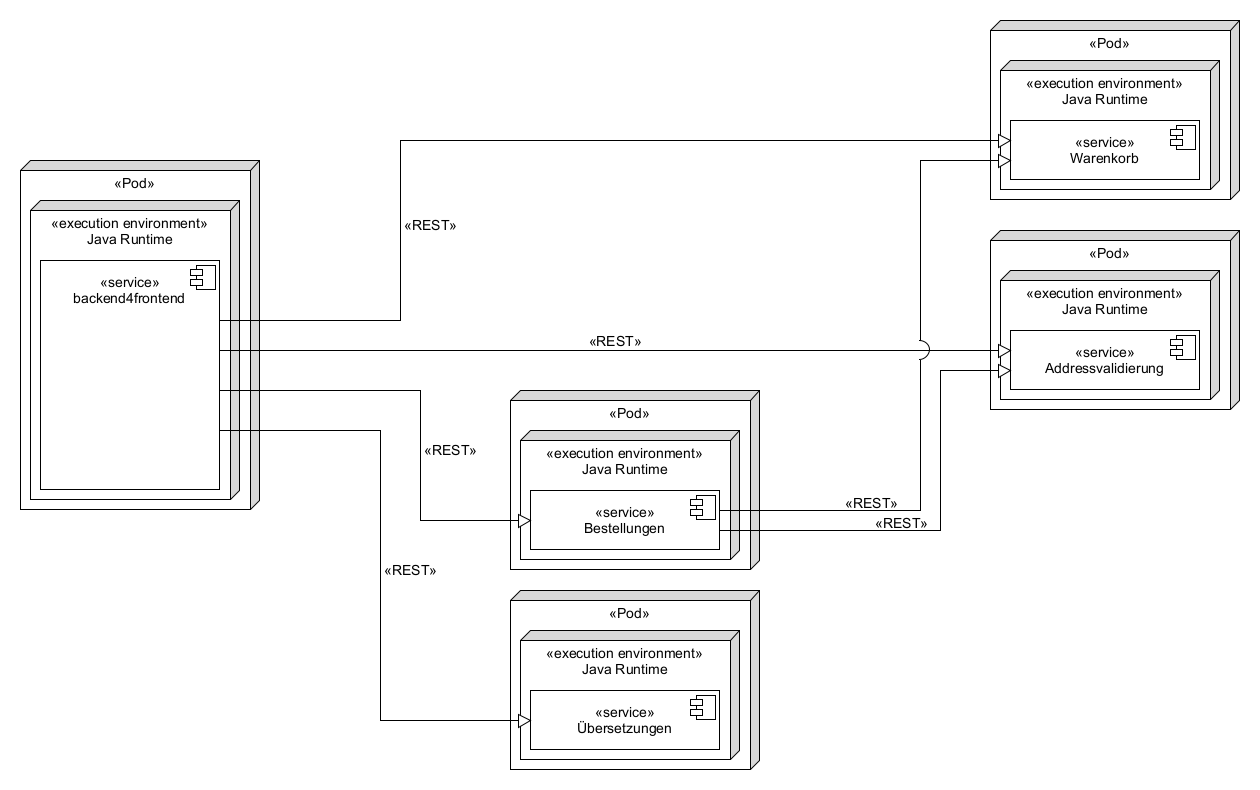
\includegraphics[width=1.00\linewidth]{img/04_erstellung-poc/demoanwendung_deployment.png}
	\caption{Demoanwendung: Deployment-Diagramm. Eigene Darstellung}
	\label{fig:demoanwendung_deployment}
\end{figure}

Die einzelnen Dienste wurden mit Eclipse MicroProfile \cite{EclipseMicroprofile} umgesetzt. MicroProfile ist eine Sammlung verschiedener Java-EE-Frameworks und Technologien zur Umsetzung von Microservices. Kern der Dienste, die auf MicroProfile basieren, sind die REST-Schnittstellen, die mit JAX-RS umgesetzt werden.

Die einzelnen Dienste wurden jeweils als Docker-Images\footnote{Docker \cite{Docker} ist eine Software zum Erstellen und Ausführen von Anwendungscontainern \cite{PatternsForSoftwareOrchestration}} gepackt, zur Gewährleistung einer einheitlichen Umgebung auch auf unterschiedlichen Rechnern. Um ein einfaches Management der Services zu ermöglichen, wird die Plattform Kubernetes\footnote{Kubernetes \cite{Kubernetes} ist eine Software zum Orchestrieren Container-basierter Anwendungen \cite{KeyCharacteristicsOfAContainerOrchestrationPlatform}} verwendet.

\subsection{Frontend}

Auf Basis von Angular realisiert das Frontend einen Wizard, welcher mehrere aufeinander folgende Formulare in derselben SPA enthält. Anhand eines Beispieldurchlaufs durch die einzelnen Seiten wird das Frontend veranschaulicht:

\begin{quotation}
	Warenkorb \textrightarrow{} Rechnungsadresse \textrightarrow{} Lieferdaten \textrightarrow{} Zahlungsdaten
	 \textrightarrow{} Bestellung abschließen \textrightarrow{} Bestellbestätigung
\end{quotation}

\subsubsection{Warenkorb}

Die erste Seite des Wizards zeigt den Inhalts des Warenkorbs eines Online-Shops für Früchte (vgl \autoref{fig:demoanwendung_vorstellung_01-warenkorb}). Hier kann der Nutzer seine Auswahl prüfen und bei Zufriedenheit kann er den Bestellvorgang starten.

Die hier angezeigten Daten werden vom Warenkorbdienst abgerufen, über die Angabe eines zuvor zufällig generierten Warenkorb-Identifiers. Die Warenkorbdaten werden zudem mit Übersetzungsdaten vom Übersetzungsdienst angereichert, denn in den Warenkorbdaten stehen lediglich Übersetzungsschlüssel wie \texttt{item.peach}, die dann auf den tatsächlichen Übersetzungswert abgebildet werden also \texttt{Pfirsich}. Beim Starten des Bestellvorgangs wird kein Serverabruf durchgeführt, sondern in der SPA wird ein Seitenwechsel vorgenommen.

\begin{figure}[H]
	\centering
	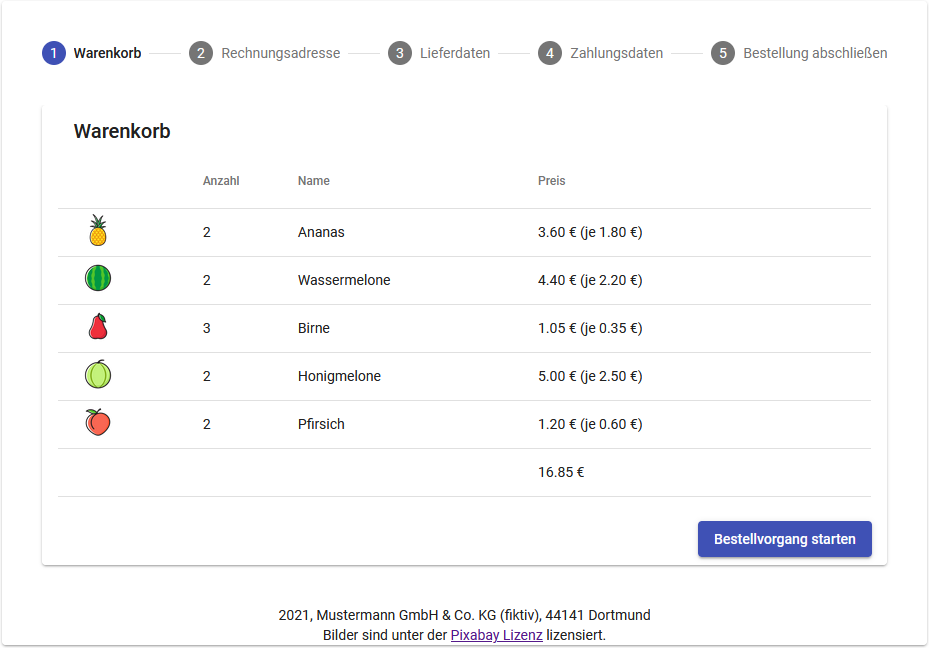
\includegraphics[width=1.00\linewidth]{img/04_erstellung-poc/demoanwendung_vorstellung_01-warenkorb_more-items.png}
	\caption{Demoanwendung: Startseite \enquote{Warenkorb}. Eigener Screenshot}
	\label{fig:demoanwendung_vorstellung_01-warenkorb}
\end{figure}

\subsubsection{Rechnungsadresse}

Auf der zweiten Seite des Wizards wird die Rechnungsadresse erfasst (vgl. \autoref{fig:demoanwendung_vorstellung_02-rechnungsadresse}). Hierbei wird der Nutzer gebeten rechnungsrelevante Informationen, wie seine Adresse, anzugeben. Er kann jedoch auch auf die vorherige Seite zurückspringen.

Beim Absenden des Formulars wird zunächst die Validität der Eingabefelder überprüft, bspw. ob die PLZ aus 5 Zahlen besteht, und anschließend wird die Adresse dem Adressvalidierungsdienst zur Prüfung übergeben. Schlägt eine Validierung fehl, so wird dies entweder direkt am verursachenden Textfeld angezeigt oder in einer allgemeinen Fehlermeldung im unteren Bereich der Eingabemaske ausgegeben.

Sind beide Prüfungen jedoch erfolgreich, so wird ein Seitenwechsel in der SPA durchgeführt. Neben der Adressüberprüfung wird kein zusätzlicher Serveraufruf abgesetzt, die eingegeben Daten werden jedoch intern einer übergeordneten Komponente übergeben.

\begin{figure}[H]
	\centering
	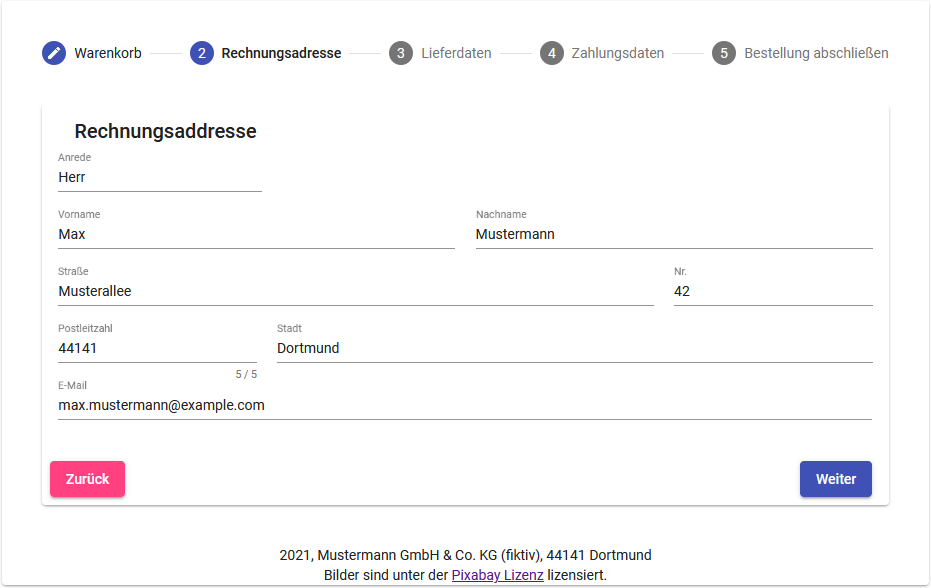
\includegraphics[width=1.00\linewidth]{img/04_erstellung-poc/demoanwendung_vorstellung_02-rechnungsadresse.png}
	\caption{Demoanwendung: Seite \enquote{Rechnungsadresse}. Eigener Screenshot}
	\label{fig:demoanwendung_vorstellung_02-rechnungsadresse}
\end{figure}

\newpage

\subsubsection{Lieferdaten}

Die dritte Seite des Wizards erfasst die Lieferdaten des Nutzers. Der Nutzer kann entweder die relevanten Daten aus der Rechnungsadresse übernehmen lassen (Standardfall) oder er gibt alternativ abweichende Lieferdaten an, wie in \autoref{fig:demoanwendung_vorstellung_03-lieferdaten} zu sehen ist. Wie zuvor kann der Nutzer auch auf das vorherige Formular zurückspringen.

Bei der Angabe von abweichenden Lieferdaten werden, wie beim Formular der Rechnungsadresse, zunächst die Eingabefelder überprüft und bei Fehlschlag visuell dem Nutzer kenntlich gemacht. Anders als bei der Rechnungsadresse wird jedoch nicht der Adressvalidierungsdienst befragt, dies wird im \autoref{subsec:ungueltige-adressen-sind-gueltig} aufgefasst und erläutert.

Sind keine abweichenden Lieferdaten erwünscht oder die Validierung der Eingaben erfolgt, wird beim Klick auf \enquote{Weiter} ein Seitenwechsel in der SPA durchgeführt. Auch hier erfolgt kein Serveraufruf, jedoch werden die Daten an die übergeordnete Komponente innerhalb der Webanwendung weitergereicht.

\begin{figure}[H]
	\centering
	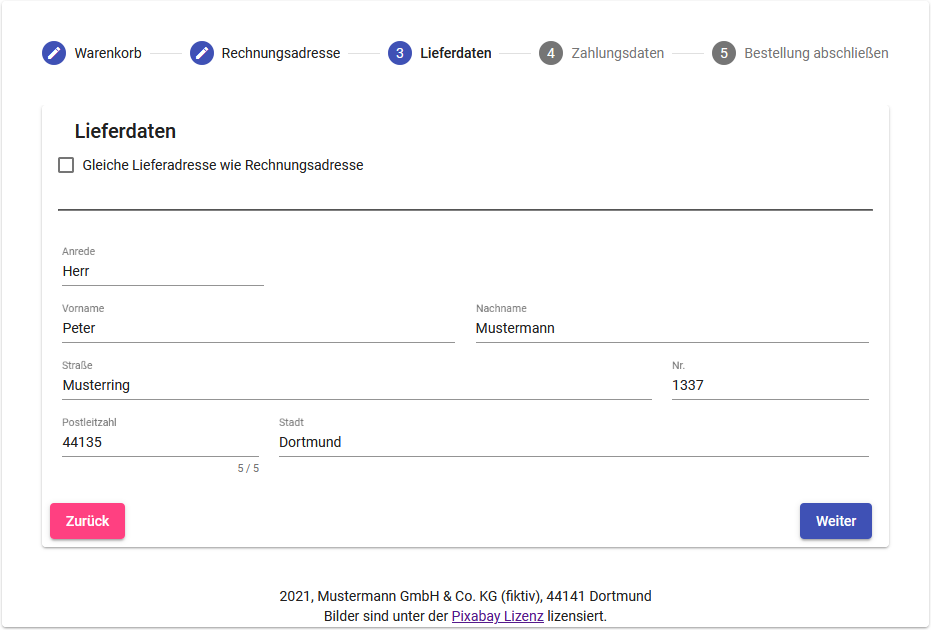
\includegraphics[width=1.00\linewidth]{img/04_erstellung-poc/demoanwendung_vorstellung_03-lieferdaten.png}
	\caption{Demoanwendung: Seite \enquote{Lieferdaten}. Eigener Screenshot}
	\label{fig:demoanwendung_vorstellung_03-lieferdaten}
\end{figure}

\subsubsection{Zahlungsdaten}

Die vierte Seite des Wizards bittet den Nutzer zur Eingabe seiner gewünschten Zahlart sowie der jew. Zahlungsinformationen. Dabei kann der er zwischen 4 Zahlungsarten wählen: per Rechnung, Lastschrift, PayPal oder Kreditkarte. Wie bei den anderen Formularen kann der Nutzer auf das vorhergehende Formular über den Button \enquote{Zurück} wechseln.

Bei Auswahl der Rechnungsart \enquote{Rechnung} muss der Nutzer keine weiteren Daten eingeben. Hingegen sind bei anderen Rechnungsarten weitere Daten einzugeben, wie z. B. der in der \autoref{fig:demoanwendung_vorstellung_04-zahlungsdaten} zu betrachteten Rechnungsart \enquote{Lastschrift}, hier muss der Kontoinhaber und die IBAN angegeben werden. Bei PayPal ist die E-Mail anzugeben und bei der Auswahl der Kreditkarte folgende Kreditkarteninformationen: Karteninhaber, Kartennummer, CVC sowie das Ablaufdatum. Die jeweilig einzugebenden Daten werden clientseitig validiert, ähnlich wie bei den vorherigen Formularen.

Ist eine Rechnungsart ausgewählt und die einzugebenden Daten valide ausgefüllt, so führt ein Absenden des Formulars zu einem Seitenwechsel auf die Seite zum Abschließen der Bestellung. Es wird keine zusätzliche Serverinteraktion durchgeführt, die Daten werden jedoch erneut an die übergeordnete Komponenten übergeben.

\begin{figure}[H]
	\centering
	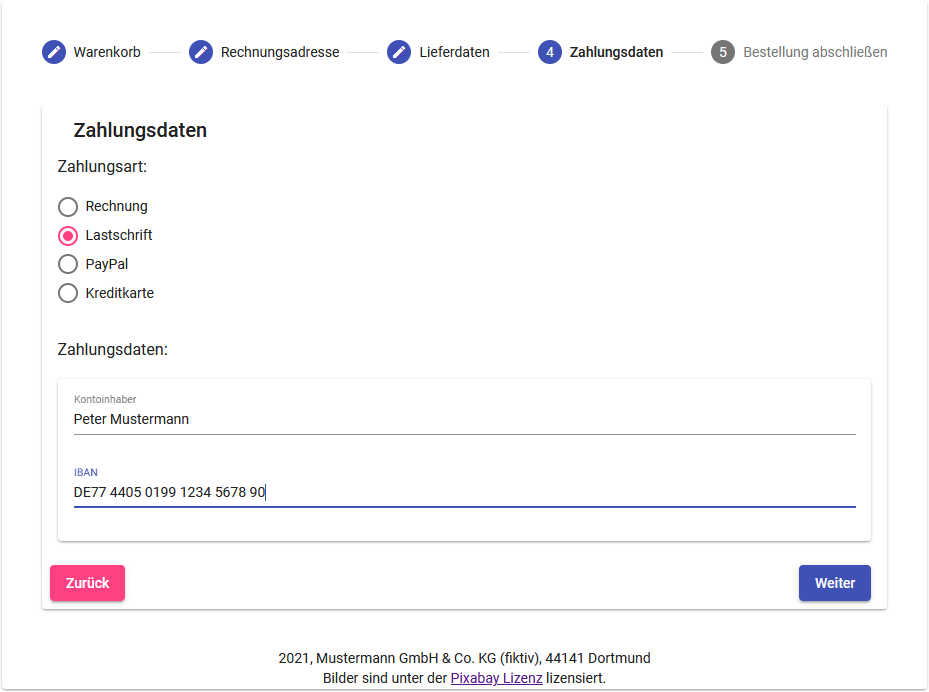
\includegraphics[width=0.85\linewidth]{img/04_erstellung-poc/demoanwendung_vorstellung_04-zahlungsdaten.png}
	\caption{Demoanwendung: Seite \enquote{Zahlungsdaten}. Eigener Screenshot}
	\label{fig:demoanwendung_vorstellung_04-zahlungsdaten}
\end{figure}

\subsubsection{Bestellübersicht}

Die vorletzte Seite des Wizard fasst die Bestelldaten zusammen (vgl. \autoref{fig:demoanwendung_vorstellung_05-bestelluebersicht}) und sendet die Daten bei der Bestätigung des Formulars an das Backend. Wie bei allen Formularen gibt es auch hier die Option für den Nutzer zu einem vorherigen Formular zurückzuspringen und Anpassungen vorzunehmen.

In der Bestellübersicht werden explizit der ausgewählte Warenkorb, die eingegebenen Rechnungs- und Lieferadresse sowie die gewählte Zahlungsart dargestellt. Der Warenkorb wird hierbei analog zur Warenkorbseite vom Warenkorbdienst abgefragt. Zuvor eingegebene Daten sind hingegen lediglich clientseitig gespeichert und werden von einer übergreifende Komponente bereitgestellt. Weitere Eingaben des Nutzers sind auf dieser Seite aber nicht gefordert, sie dient hauptsächlich der visuellen Überprüfung für den Nutzer bevor er die Bestellung kostenpflichtig durchführt.

Sendet der Nutzer die Bestellung ab, werden die zuvor eingegeben Daten und der Identifier des Warenkorbs an den Bestelldienst übergeben. Dieser überprüft beide Adresseingaben gegen den Adressvalidierungsdienst, ruft den Warenkorb vom Warenkorbdienst ab und errechnet auf dieser Datenbasis den Bestellbeleg. Der Bestellbeleg wird dem Frontend in der Antwort übergeben, weiterhin erfolgt ein Seitenwechsel.

\begin{figure}[H]
	\centering
	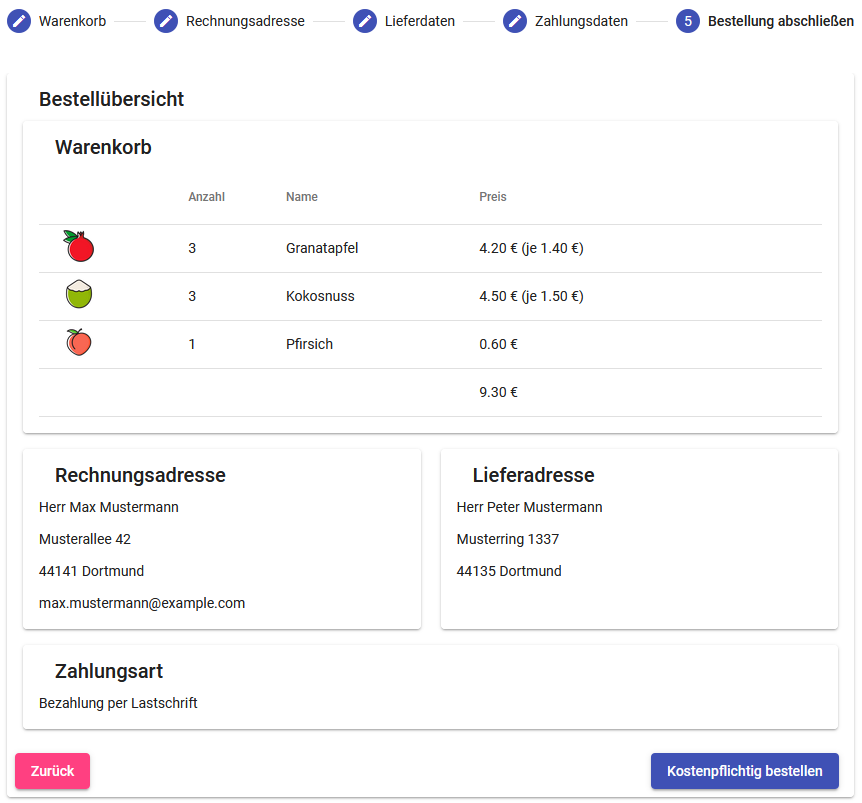
\includegraphics[width=0.68\linewidth]{img/04_erstellung-poc/demoanwendung_vorstellung_05-bestelluebersicht_cropped}
	\caption{Demoanwendung: Seite \enquote{Bestellübersicht}. Eigener Screenshot}
	\label{fig:demoanwendung_vorstellung_05-bestelluebersicht}
\end{figure}

\subsubsection{Bestellbestätigung}

Die sechste und letzte Seite des Wizards visualisiert die Bestellbestätigung nach einer erfolgreichen Bestellung, wie in \autoref{fig:demoanwendung_vorstellung_06-bestellbestaetigung} zu sehen ist. Bei den angezeigten Daten handelt es sich nicht um die zuvor gespeicherten, sondern ausschließlich um die vom Bestelldienst übermittelten Daten.

Auf dieser Seite kann der Nutzer nun nur noch auf den Button \enquote{Zum Shop} klicken und gelangt erneut zur Startseite, jedoch mit einem neuen Warenkorb.

\begin{figure}[H]
	\centering
	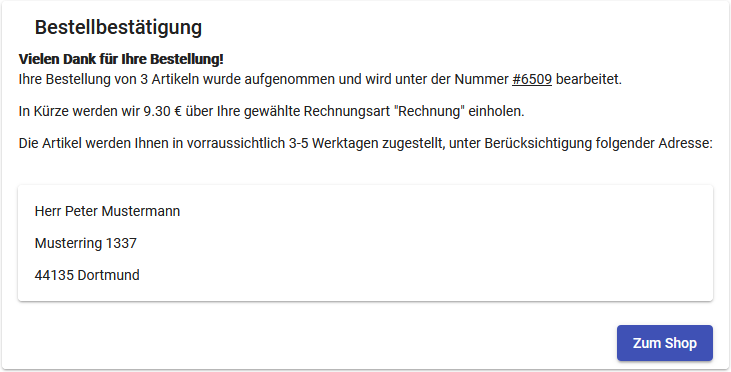
\includegraphics[width=0.75\linewidth]{img/04_erstellung-poc/demoanwendung_vorstellung_06-bestellbestaetigung.png}
	\caption{Demoanwendung: Finale Seite \enquote{Bestellbestätigung}. Eigener Screenshot}
	\label{fig:demoanwendung_vorstellung_06-bestellbestaetigung}
\end{figure}

\subsection{Fehlerszenarien}
\label{subsec:fehlerszenarien}

Um später mithilfe von Observability-Werkzeugen Probleme aufzudecken und Aspekte der Nachvollziehbarkeit darzustellen, weist die Demoanwendung eine Reihe von typischen Fehlern auf, die bewusst integriert wurden.

Diese Fehler gehören unterschiedlichen Problemgruppen an, sie reichen von unerwünscht strenger Validierung, über Konfigurationsfehlern bis hin zu ineffizienter Datenverarbeitung. Ein Ausschnitt wird folgend in Fehlerszenarien beschrieben, aus der Sicht eines Projektteams, welches diese Szenarien berichtet bekommen oder selbst notiert hat.

\pagebreak

\subsubsection{\enquote{Keine Übersetzungen}}
\label{subsec:keine-uebersetzungen}

\begin{wrapfigure}[7]{r}{0.33\textwidth}
\centering
\vspace{-\baselineskip}
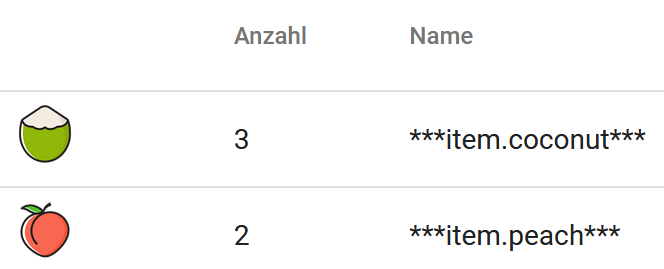
\includegraphics[width=\linewidth]{img/04_erstellung-poc/demoanwendung_fehlerszenario-uebersetzungen}
\caption{Fehlende Texte. Eigener Screenshot}
\label{fig:demoanwendung_fehlerszenario-uebersetzungen}
\end{wrapfigure}

- Problem: Nutzer berichten, dass manchmal die Webanwendung beim Start keine Artikeltexte anzeigt (vgl \autoref{fig:demoanwendung_fehlerszenario-uebersetzungen}).

- Ursache: Die Pods, die den Übersetzungsdienst enthalten, werden repliziert bereitgestellt. Einer der Pods hat eine defekte Konfiguration, weswegen er keine Übersetzungen der Artikel enthält. Wird zu diesem Pod verbunden, tritt das Fehlverhalten auf. Dies ist eine Nachstellung eines tatsächlichen Problems beim Kunden.

%\subsubsection{\enquote{Gültige Straßen sind ungültig}}
%
%- Problem: Nutzer berichten, dass Ihr Straßenname nicht eingeben werden kann. Beispielsweise führt die Eingabe \enquote{Ährenweg} zu einem Fehler.
%
%- Ursache: Der Adressvalidierungsdienst validiert Straßen mit dem Regular-Expression \texttt{[a-zA-Z\textbackslash,\textbackslash-\textbackslash ]+}, welches keine gängigen Sonderzeichen (ä ,ö ,ü, ß) erlaubt.

% rausgenommen, zu viel Dopplung
%\subsubsection{\enquote{Gültige Hausnummern sind ungültig}}
%
%- Problem: Nutzer berichten, dass Hausnummern, die nicht nur aus Zahlen bestehen, zum Fehler führen.
%
%- Ursache: Der Adressvalidierungsdienst validiert Hausnummern als Zahl und schlägt im o. g. Fall in der Konvertierung fehl.

%\subsubsection{\enquote{Gültige Städte sind ungültig}}
%
%- Problem: Nutzer aus Gießen berichten, dass Sie das Formular zur Rechnungsadresse nicht ausfüllen können
%
%- Ursache: Der Adressvalidierungsdienst meldet die Stadt \enquote{Gießen} als ungültig, weil sie nicht in der lokalen Tabelle vorhanden ist.

\subsubsection{\enquote{Ungültige Adressen sind gültig}}
\label{subsec:ungueltige-adressen-sind-gueltig}

- Problem: Nutzer können in den Lieferdaten ungültige Eingaben tätigen und absenden, bei der Bestellaufgabe kommt es zu einem Fehler.

- Ursache: Das Frontend überprüft lediglich die Rechnungsadresse, aber nicht die Lieferadresse

%\subsubsection{\enquote{Vor- und Nachnamen werden abgeschnitten}}
%
%- Problem: Nutzer berichten, dass in der Bestellbestätigung Ihre Vor- und Nachnamen abgeschnitten dargestellt werden.
%
%- Ursache: Der Bestelldienst begrenzt den Vor- sowie den Nachnamen auf 20 Zeichen, das Frontend begrenzt dies jedoch nicht.

%\subsubsection{\enquote{Falsche Zahlungsart}}
%
%- Problem: Nutzer berichten, dass in der Bestellbestätigung die falsche Zahlungsart angezeigt wird. In der Bestellübersicht wurde jedoch die korrekte Zahlungsart angezeigt.
%
%- Ursache: Das Frontend sendet alle Formulardaten jeder Rechnungsart an den Dienst \enquote{Bestellungen}. Dieser nimmt aber an, dass alle nicht ausgewählten Rechnungsarten statt Formulardaten nur \texttt{null} enthalten.

\subsubsection{\enquote{Lange Verarbeitung}}
\label{subsec:lange-verarbeitung}

- Problem: Beim Abrufen der Warenkorbdaten kommt es zu einer unerwünschten Wartezeit (von ca. 6-10s).

- Ursache: Dies ist eine simulierte Wartezeit im Frontend, hierbei wird eine ineffiziente Mapping-Operation nachgeahmt.

%\subsection{Repräsentation}
%
%Eine wichtige Eigenschaft der Demoanwendung sollte sein, dass sie repräsentativ für die Webanwendung des Kunden ist und im Allgemeineren auch für moderne Webanwendungen ist. Durch den groben Aufbau der Demoanwendung, also einer zustandsreichen und zu großen Teilen clientbasierten SPA, stellt die Demoanwendung eine moderne Webanwendung dar. Auch die Verwendung von Angular ist repräsentativ, denn Angular ist eines der meist verwendeten Frontend-Frameworks \cite{TheStateOfJavaScript2020}.
%
%Das Backend ist in dem Sinne repräsentativ, dass es auf keiner stark vereinfachten Infrastruktur basiert, sondern gewollt an die Situation des Open Knowledge Kunden abbildet. Des Weiteren stellt die gewählte Architektur einen modernen Ansatz dar, denn die Architektur ist Microservice-orientiert \cite{MicroserviceArchitecture}.

\subsection{Repräsentation}

Es ist anzumerken, dass die Demoanwendung nur ein Modell einer tatsächlichen Webanwendung darstellt. Wie jedes Modell können nicht alle Gegebenheiten des zu modellierenden Sachverhalts nachgestellt werden. Jedoch ist durch den allgemein gehaltenen Anwendungsfall und die moderne Umsetzung eine Übertragbarkeit zu ähnlichen Projekten durchaus vorhanden.

Nun da die Demoanwendung beschrieben ist, werden die Anforderungen näher erläutert, die das zu erstellende Proof-of-Concept erfüllen soll.

\pagebreak
	
\section{Anforderungen}
%\section{Anforderungen}
%\textit{Hier soll definiert werden, welche Kriterien der PoC erfüllen soll und wenn möglich sollen zusätzlich Möglichkeiten zur Überprüfung dieser Kriterien definiert werden.}

Das zu erstellende Proof-of-Concept soll einige Rahmenbedingungen erfüllen. In diesem Abschnitt werden diese Bedingungen näher beschrieben.
	
\subsection{Definitionen}
	
Um die Anforderungen systematisch einzuordnen, werden folgend zwei Modelle vorgestellt, anhand dessen die Kategorisierung erfolgt.

Beim ersten Modell handelt es sich um das Kano-Modell \cite{KanoModell} der Kundenzufriedenheit, welches in  \autoref{tab:merkmale-nach-dem-kano-modell} erläutert wird.
	
\begin{table}[H]
\begin{tabular}{ |p{1.15cm}|p{2.75cm}|p{9.6cm}| }
	\hline
	Kürzel & Titel & Beschreibung \\
	\hline
	\textbf{B} & Basis\-merkmal & Merkmale, die als selbstverständlich angesehen werden. Eine Erfüllung erhöht kaum die Zufriedenheit, jedoch eine Nichterfüllung führt zu starker Unzufriedenheit \\
	\hline
	\textbf{L} & Leistungs\-merkmal & Merkmale, die der Kunde erwartet und bei nicht Vorhandensein in Unzufriedenheit äußert. Ein Vorhandensein erzeugt Zufriedenheit, beim Übertreffen umso mehr. \\
	\hline
	\textbf{S} & Begeisterungs\-merkmal & Merkmale, die eine Herabsetzung von der Konkurrenz ermöglichen und die den Nutzenfaktor steigern. Sind sie vorhanden, steigern sie die Zufriedenheit merklich. \\
	\hline
	\textbf{U} & Unerhebliches Merkmal & Für den Kunden belanglos, ob vorhanden oder nicht. \\
	\hline
	\textbf{R} & Rückweisungs\-merkmal & Diese Merkmale führen bei Vorhandensein zu Unzufriedenheit, sind jedoch beim Fehlen unerheblich. \\
	\hline
\end{tabular}
 \captionsetup{justification=centering}
  \caption{Merkmale nach dem Kano-Modell der Kundenzufriedenheit}
   \label{tab:merkmale-nach-dem-kano-modell}
\end{table}

Neben der Unterscheidung nach dem Kano-Modell werden die Anforderungen in funktionale und nicht-funktionale Anforderungen \cite{FunktionaleUndNichtFunktionaleAnforderungen} aufgeteilt (vgl. \autoref{tab:kategorien-der-anforderungsliste}).

\begin{table}[H]
\begin{tabular}{ |p{1.15cm}|p{2.75cm}|p{9.6cm}| }
	\hline
	Kürzel & Titel & Beschreibung \\
	\hline
	f & funktional & Beschreiben Anforderungen, welche ein Produkt ausmachen und von anderen differenzieren (\enquote{Was soll das Produkt können?}). Sie sind sehr spezifisch für das jeweilige Produkt. Ein Beispiel: Das Frontend fragt Daten für X vom Partnersystem 1 über eine SOAP-API ab, etc.\\
	\hline
	nf & nicht-funktional & Beschreiben Leistungs- und Qualitätsanforderungen und Randbedingungen (\enquote{Wie soll das Produkt sich verhalten?}). Sie sind meist unspezifisch und in gleicher Form auch in unterschiedlichsten Produkten vorzufinden. Beispiele sind: Benutzbarkeit, Verfügbarkeit, Antwortzeit, etc. Zur Überprüfung sind oftmals messbare, vergleichbare und reproduzierbare Definitionen notwendig. \\
	\hline
\end{tabular}
 \captionsetup{justification=centering}
  \caption{Kategorien der Anforderungen}
   \label{tab:kategorien-der-anforderungsliste}
\end{table}
	
\subsection{Anforderungsanalyse}

Die Anforderungen, welche von der zu erstellende Lösung gefordert werden, ergaben sich durch den Einfluss verschiedener Quellen. Die primäre Quelle an Anforderungen stellen die Stakeholder dieser Arbeit, Christian Wansart und Stephan Müller, dar. Als Stakeholder betreuen sie die Arbeit und haben ein eigenes Interesse, dass aus der Arbeit ein erfolgreiches und übertragbares Ergebnis resultiert.

Neben den Stakeholdern ergeben sich auch Anforderungen direkt aus der Forschungsfrage selbst und den Bestrebungen des Autors. Die Quellen werden in den Anforderungen mit einem Kürzel angegeben, wie z. B. \texttt{A} für Autor, zu sehen in \autoref{tab:quellen-der-anforderungen}.

Eine dritte Quelle von Anforderungen ergibt sich aus der Problemstellung des Kunden der Open Knowledge, welche in der Motivation angesprochen wurde. Die beiden Stakeholder brachten neben ihren eigenen Bestrebungen auch die Rahmenbedinungen und Wünsche des Kunden mit ein. Aus dieser Kommunikation ergaben sich somit weitere Anforderungen, welche einen realitätsnahen Charakter haben.

Anforderungen können auch eine Kombination von mehreren Quellen besitzen, wenn die Anforderung aus einer gemeinsamen Bestrebung oder Diskussion entstand.

\begin{table}[H]
\begin{tabular}{ |p{1.15cm}|p{1.9cm}|p{10.45cm}| }
	\hline
	Kürzel & Titel & Beschreibung \\
	\hline
	A & Autor & Hiermit ist der Autor dieser Arbeit gemeint. \\
	\hline
	S & Stakeholder & Die beiden Stakeholder Christian Wansart und Stephan Müller \\
	\hline
	K & Kunde & Ein Kunde der Open Knowledge, ein Direktversicherer. \\
	\hline
\end{tabular}
 \captionsetup{justification=centering}
  \caption{Quellen der Anforderungen}
   \label{tab:quellen-der-anforderungen}
\end{table}
	
\subsection{Anforderungsliste}

Um die Anforderungen strukturiert zu erfassen, werden sie ähnlich einer Karteikarte, wie in \autoref{tab:beispiel-anforderung} zu sehen, dargestellt. Hierbei erhält jede Anforderung eine Kategorisierung nach dem Kano-Modell, ob sie funktional oder nicht-funktional ist und aus welcher Anforderungsquelle sie entstammt. Jede Anforderung erhält zudem eine eindeutige Id, die nachfolgend in der Arbeit zur Referenzierung dient.

\begin{table}[H]
\begin{tabular}{ |p{1.25cm}|p{5.5cm}|p{2.25cm}|p{2.1cm}|p{1.25cm}| }
\hline
Id            & Name          & Kano-Modell   & Funktionsart  & Quelle        \\
\textit{1234} & \textit{Dummy} & \textit{S} & \textit{nf} & \textit{S} \\
\hline
\multicolumn{5}{|l|}{\textit{Hier wird die Anforderung beschrieben.}} \\
\hline
\end{tabular}
 \captionsetup{justification=centering}
  \caption{Beispiel einer Anforderung}
   \label{tab:beispiel-anforderung}
\end{table}

% use generated list

% textidote: ignore begin

\subsubsection{Grundanforderungen}


\subsubsection{Funktionsumfang}


\begin{anf}{anf:1010}{1010}{Schnittstellen-Logging}{B}{f}{S}
\multicolumn{5}{|p{14.05cm}|}{Das Aufrufen von Schnittstellen soll mittels einer Logmeldung notiert werden. Hierbei sollen relevante Informationen wie Aufrufparameter mit notiert werden.} \\
\hline
\end{anf}

\begin{anf}{anf:1011}{1011}{Use-Case-Logging}{B}{f}{S}
\multicolumn{5}{|p{14.05cm}|}{Tritt ein Use-Case auf, soll dieser im Log notiert werden. Beispielsweise soll notiert werden, dass ein Nutzer einen neuen Datensatz angelegt möchte und wenn der diesen anlegt.} \\
\hline
\end{anf}

\begin{anf}{anf:1100}{1100}{Logübertragung}{B}{f}{S}
\multicolumn{5}{|p{14.05cm}|}{Ausgewählte Logmeldungen sollen an ein Partnersystem weitergeleitet werden. Die Auswahl könnte über die Kritikalität, also dem Log-Level, der Logmeldung erfolgen.} \\
\hline
\end{anf}

\subsubsection{Eigenschaften}


\begin{anf}{anf:2010}{2010}{Resilienz der Übertragung}{S}{f}{S}
\multicolumn{5}{|p{14.05cm}|}{Daten die der Nachvollziehbarkeit dienen, sollen wenn möglich bei einer fehlgeschlagenen Verbindung nicht verworfen werden. Sie sollen mindestens 120s vorgehalten werden und in dieser Zeit sollen wiederholt Verbindungsversuche unternommen werden.} \\
\hline
\end{anf}

\begin{anf}{anf:2020}{2020}{Batchverarbeitung}{S}{f}{S}
\multicolumn{5}{|p{14.05cm}|}{Daten, die der Nachvollziehbarkeit dienen, sollen wenn möglich gruppiert an externe Systeme gesendet werden. Hierbei ist eine kurze Aggregationszeit von bis zu 10s akzeptabel.} \\
\hline
\end{anf}

\subsubsection{Partnersysteme}

% textidote: ignore end
	
\section{Konzept}
	
	\subsection{Datenverarbeitung}

	Auf Basis der zuvor vorgestellten Methoden und Praktiken wird nun eine sinnvolle Kombination für das Frontend konzeptioniert, die als Ziel hat, die Nachvollziehbarkeit nachhaltig zu erhöhen. Es werden die Grunddisziplinen Datenerhebung, -auswertung und -präsentation unterschieden und nacheinander beschrieben. Danach und darauf aufbauend wird eine grobe Architektur vorgestellt, die diese Ansätze in ein Gesamtbild bringt.
		
	\subsubsection{Erhebung}
	
	Wie zuvor in \autoref{sec:nachvollziehbarkeit-bei-spas} beschrieben, erhalten Betreiber und Entwickler im Normalfall nur unzureichende Information über das Anwendungsverhalten oder die getätigten Nutzerinteraktionen bei einer SPA. Aus diesem Grund sollen explizit weitere Daten erhoben werden, um die Nachvollziehbarkeit zu erhöhen.
	
	Wie aus den Erkenntnissen von FAME (\autoref{sec:fame}) und Kaiju (\autoref{sec:kaiju}) zu deuten ist, gibt es durch die Verknüpfung von verschiedenen Datenkategorien einen Mehrwert für die Verständnis von Betreibern und Entwicklern. Deshalb sollen in der Lösung die 4 Datenkategorien \enquote{Logs}, \enquote{Metriken}, \enquote{Traces} und \enquote{Fehler} erhoben und an Partnersysteme weitergeleitet werden.
	
	Neben diesen Daten sollen auch die Benutzerinteraktionen aufgezeichnet werden. Hierfür soll jedoch kein tiefer gehendes Real-User-Monitoring zur Verwendung kommen, stattdessen soll ein Session-Replay-Mechanismus eingesetzt werden. RUM wird nicht gefordert, da es für die Verständnisgewinnung der Benutzerinteraktionen weniger aussagekräftig ist als Session-Replay. Bei Session-Replay werden die Benutzerinteraktionen im Kontext dargestellt und nicht gesondert oder abstrahiert, was für eine Nachvollziehbarkeit hinderlich sein kann. Beim Session-Replay wird jedoch jedwede Ein- und Ausgaben der Webanwendung aufgezeichnet, damit dies nicht ein zu großes Datenvolumen erzeugt und um den Nutzer nicht konstant zu überwachen, sollte sie standardmäßig abgeschaltet sein und nur auf expliziten Nutzerwunsch aktiviert werden.
	
	\vspace{-0.75\baselineskip}
	\subsubsection{Auswertung}
	\vspace{-0.50\baselineskip}
	
	Die genaue Auswertung ist Teil der Implementierung und diese Disziplin sieht keine direkten Vorgaben vor. Jedoch sind die gemeldeten Daten mit Kontextinformationen anzureichern, wenn möglich. Diese umfassen bspw. Zeitstempel, User-Agent, IP, Browser.
	
	\vspace{-0.75\baselineskip}
	\subsubsection{Präsentation}
	\vspace{-0.50\baselineskip}
	
	Um ein zufriedenstellendes Ergebnis zu gewährleisten, sollte die Lösung die Daten auf folgende Weise den Betreibern und Entwicklern präsentieren:
	
	\begin{enumerate}
		\item Logdaten..
		\begin{enumerate}
			\item ..lassen sich einsehen.
			\item ..lassen sich basierend auf ihren Eigenschaften filtern.
		\end{enumerate}
		\item Fehler..
		\begin{enumerate}
			\item ..lassen sich einsehen,
			\item ..lassen sich basierend auf ihren Eigenschaften filtern,
			\item ..lassen sich gruppieren.
			\item Fehlergruppen lassen sich in Graphen visualisieren (bspw. Histogramm der Häufigkeit).
		\end{enumerate}
		\item Metriken..
		\begin{enumerate}
			\item ..lassen sich in Graphen visualisieren.
		\end{enumerate}
		\item Traces..
		\begin{enumerate}
			\item ..lassen sich einsehen,
			\item ..lassen sich basierend auf ihren Eigenschaften filtern,
			\item ..lassen sich als ein Trace-Gantt-Diagramm darstellen.
		\end{enumerate}
		\item Session-Replay-Daten
		\begin{enumerate}
			\item Mithilfe der Session-Replay-Daten soll eine videoähnliche Nachstellung einer Sitzung erstellt werden.
		\end{enumerate}
	\end{enumerate}
	
	\subsection{Architektur}
	
	Auf Basis der zuvor beschriebenen Grunddisziplinen wird nun eine beispielhafte Umsetzung dessen konzipiert. Genauer wird eine Architektur vorgeschlagen, welche auf die zuvor betrachteten Methoden und Praktiken zurückgreift, um eine verbesserter Nachvollziehbarkeit zu erreichen. Speziell wird im Folgeabschnitt zudem vorgeschlagen, welche Werkzeuge oder Technologien zum Einsatz kommen sollen und wie diese Komponenten miteinander kommunizieren.
	
	 Die genaue Erhebung der Daten ist Teil der Implementierung und wird hier nicht näher bestimmt. Jedoch ergeben sich aus der zuvor definierten Anforderungen zur Erhebung bereits Datenkategorien, welche von einem entsprechenden Partnersystem zu konsumieren und verarbeiten sind. Es wird zwar nicht auf spezielle Werkzeuge oder Technologien eingegangen, aber es lassen sich bereits Partnersysteme bestimmen, auf Basis der zuvor identifizierten Funktionsbereiche. Hierbei wurde zudem versucht möglichst viele Bereiche über die gleichen Partnersysteme abzubilden (vgl. \autoref{anf:3100}), die Machbarkeit einer solchen Verknüpfung basiert auf den Ergebnissen von \autoref{chap:methoden-und-praktiken}.
	 
	 So soll für die Verarbeitung von Fehler-, Log-, und Metrikdaten ein einzelnes Partnersystem verantwortlich sein, welches ermöglicht diese zu konsumieren, speichern, durchsuchen und diese zu visualisieren. Grund hierfür ist, dass die Daten gemeinsame Eigenschaften besitzen, die eine gemeinsame Verarbeitung erlauben. In der \autoref{fig:grobe-architektur} ist dieses System als \enquote{Log- und Monitoringplattform} vorzufinden.
	
	Um Traces zu konsumieren und den Betreibern und Entwicklern aufbereitet zu visualisieren, soll ein weiteres Partnersystem eingesetzt werden. Dieses System wurde als notwendig empfunden, da kein Werkzeug identifiziert werden konnte, welches neben Traces noch andere Datenkategorien zufriedenstellend abdecken kann. Auf Basis von OpenTelemetry könnten sich jedoch in Zukunft Technologien entwickeln, welches alle 3 Datenkategorien von OpenTelemetry unterstützt: Metriken, Traces und Logs. Es wurde sich zudem gegen eine weitreichende Monitoringplattform, wie z. B. New Relic oder Dynatrace, entschieden, denn hier wurde identifiziert, dass diese nicht ausreichend flexibel für verschiedene Projekte sind und zudem auch nicht erlauben, dass einzelne Komponenten ausgetauscht oder entfernt werden können.
	
	Es ist zudem ein drittes System notwendig, um die gewünschte Funktionalität des Session-Replays einzubinden. Session-Replay ist ein spezielles und sehr konkretes Aufgabengebiet und es konnte kein Werkzeug identifiziert werden, welches sich nicht nur auf dieses Gebiet spezialisiert.
	
\begin{figure}[H]
	\centering
	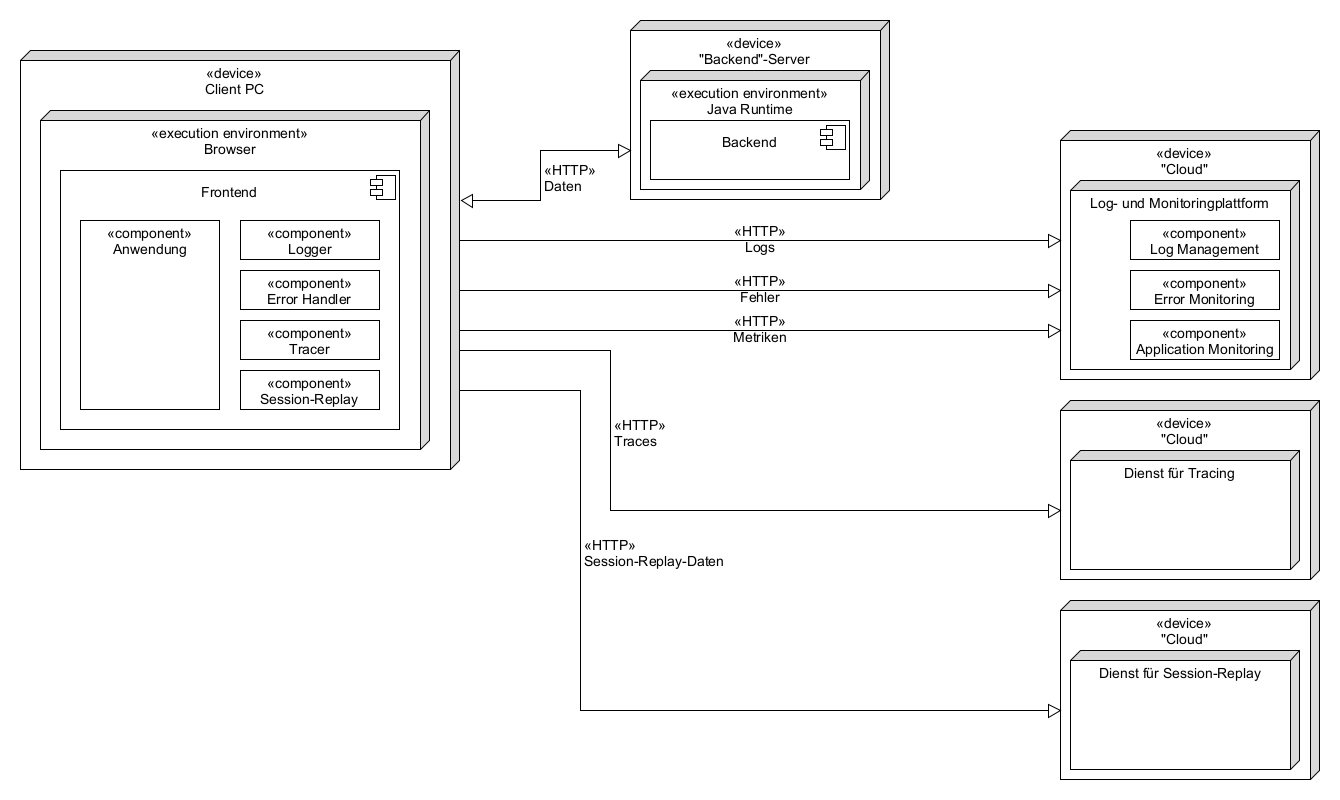
\includegraphics[width=1.00\linewidth]{img/04_erstellung-poc/konzept-simple.png}
	\caption{Grobe Architektur}
	\label{fig:grobe-architektur}
\end{figure}

%Wie in der Datenerfassung erwähnt, werden die einzelnen Datentypen unterschiedlich erhoben und besitzen somit auch andere Eigenschaften. Wie bei Big Data \cite{ZikopoulosUnderstandingBigData}, lassen sich auch hier die Eigenschaften Volume, Velocity und Variety identifizieren. Der Aspekt Volume ist weniger präsent, denn die Datenmengen sind nicht vergleichbar mit echten Big-Data-Anwendungen. Genau ist dies nicht prognostizierbar, aber in der Evaluierung des Stands der Technik, ließ sich ein Datendurchsatz von 1 MB/min feststellen - somit stellt dies im Frontend keine Herausforderung dar, jedoch in den verarbeitenden Systemen kann dies natürlich durch eine große Menge an Frontends multipliziert werden, was jedoch nicht im Fokus der Arbeit steht.
%
%Eine Variety der Daten, also Unterschiedlichkeit der Datenstruktur, ist definitiv vorhanden und entspringt den verschiedenen Funktionsgebieten. Auch innerhalb derselben Datenströme kann eine Variety identifiziert werden, denn bspw. sind Logmeldungen sehr individuell, sie folgen meist nicht streng einem Format und enthalten unterschiedliche Mengen an Informationen.
%
%Der Aspekt des Velocity ist zudem auch sehr wichtig und eine Visualisierung dessen für das vorhergehende Konzept findet sich in \autoref{fig:grobe-architektur-datendurchsatz}.
%	
%\begin{figure}[H]
%	\centering
%	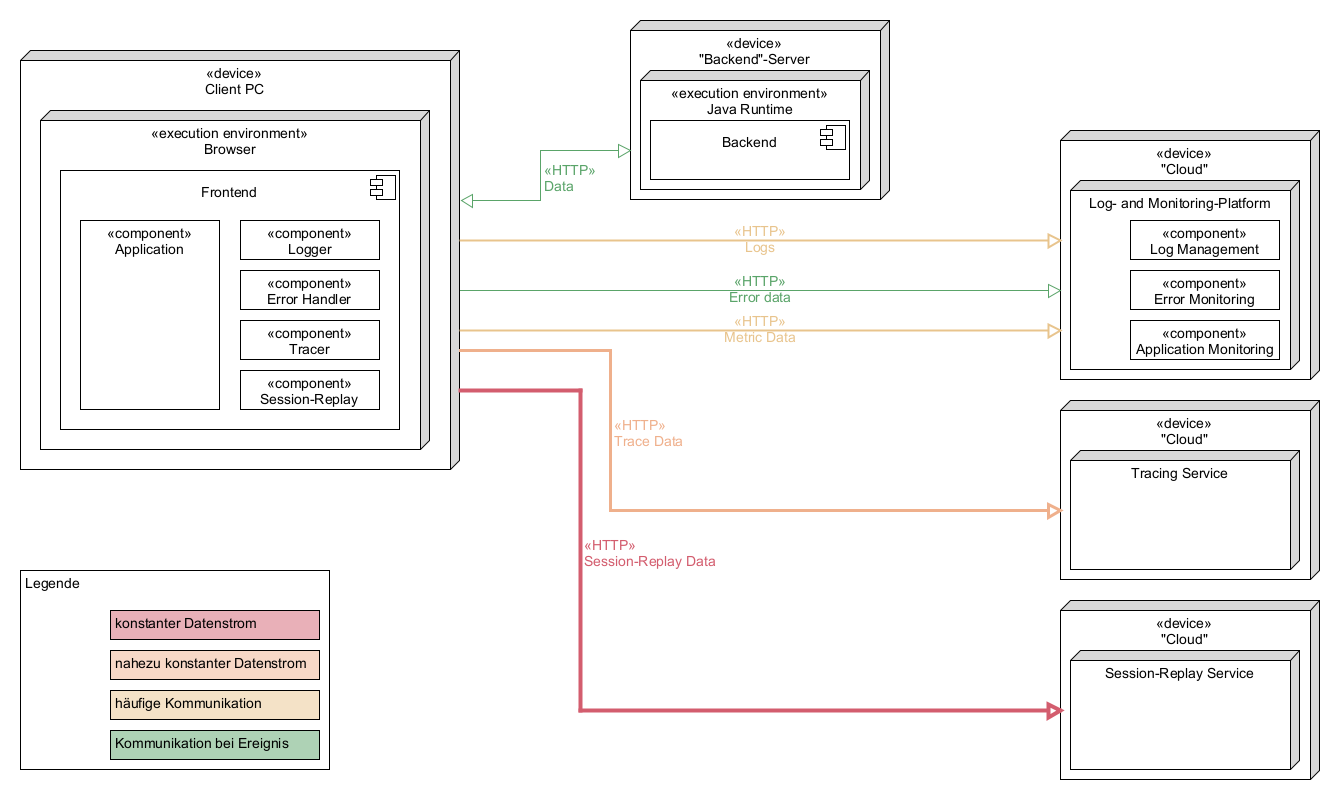
\includegraphics[width=0.75\linewidth]{img/04_erstellung-poc/konzept-datendurchsatz.png}
%	\caption{Grobe Architektur mit hervorgehobenem Datendurchsatz}
%	\label{fig:grobe-architektur-datendurchsatz}
%\end{figure}

	\subsection{Technologie-Stack}
	\label{sec:technologie-stack}
	
	Auf Basis der zuvor erstellten Architektur wird sich nun für spezielle Technologien entschieden, mit der diese Architektur umgesetzt werden soll. Weiterhin wird behandelt, wie die Daten vom Frontend aus erhoben werden sollen und wie sie an die Partnersysteme gelangen.
	
	Für die \enquote{Log- und Monitoringplattform} wurde sich für Splunk entschieden, denn auf Basis der Evaluierung konnte festgestellt werden, dass Splunk die drei gewünschten Datenkategorien Logs, Metriken und Fehler zufriedenstellend unterstützt. Es wurde sich gegen New Relic und Dynatrace entschieden, da es diesen Werkzeugen an Flexibilität fehlt und sie viele Funktionen anbieten, die für die Lösung nicht notwendig sind. Eine weitere Alternative ist der Elastic Stack, welcher jedoch nicht näher evaluiert wurde. Somit wird Splunk eingesetzt, aber für eine äquivalente Lösung kann Splunk durch ein gleichwertiges Werkzeug ausgetauscht werden.
	
	Für das Partnersystem, welches sich mit den Tracedaten befasst, wurde sich für Jaeger entschieden. Die Entscheidung wurde auf der Basis getroffen, dass Jaeger einen moderner Tracingdienst darstellt, welcher zudem quelloffen entwickelt wird. Weiterhin ist in Zukunft eine Unterstützung des OpenTelemetry-Standards geplant, was durch die standardisierte Schnittstelle die Anbindung an bestehende Systeme vereinfachen wird. Des Weiteren erfüllt Jaeger alle aufgestellten Kriterien und erzeugt zudem ein Abbild der Systemarchitektur auf Basis der Traces.
	
	Um die Session-Replay-Funktionalität einzubringen wird in diesem Konzept LogRocket vorgeschlagen. LogRockets Nachstellung einer Sitzung ist nicht nur wie gefordert videoähnlich, sondern auch interaktiv. Die gesamte HTML-Struktur wird nachgestellt und kann so zu jedem Zeitpunkt begutachtet werden.
	
	Der sich daraus ergebende Technologiestack, angewandt auf die Architektur, ist in \autoref{fig:architektur-technologien} zu betrachten. Wie bei Splunk erwähnt sind auch die anderen Werkzeuge durch gleichwertige Werkzeuge ersetzbar, so können individuelle Anpassungen erfolgen und betriebliche Gegebenheiten zu berücksichtigen.
	
\begin{figure}[H]
	\centering
	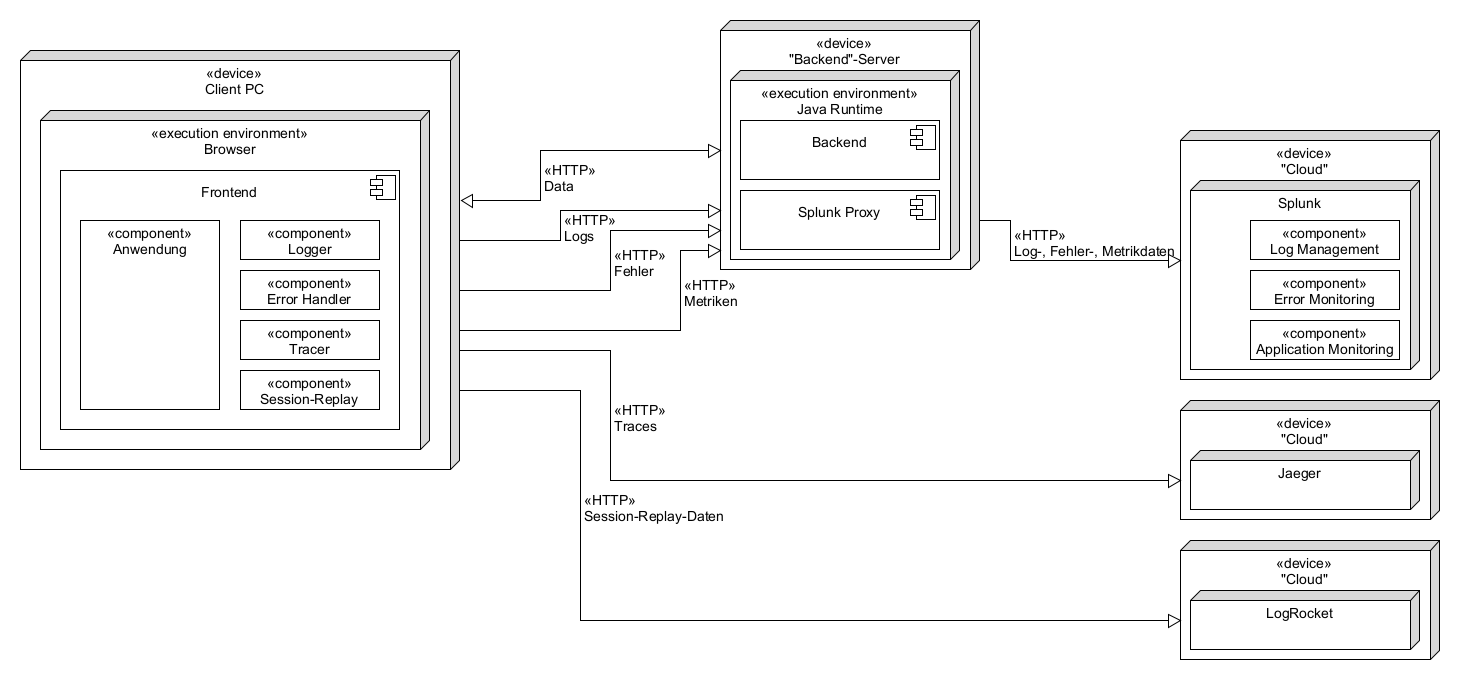
\includegraphics[width=1.00\linewidth]{img/04_erstellung-poc/konzept-technologien.png}
	\caption{Architektur mit speziellen Technologien}
	\label{fig:architektur-technologien}
\end{figure}

	\subsection{Übertragbarkeit}
	
	Übertragbarkeit beschäftigt sich mit der Eigenschaft eines Ansatzes in verschiedene Situationen anwendbar zu sein. Ein Ansatz ist nicht übertragbar, wenn zu vielen Annahmen über die Situation getroffen werden.
	
	Das zuvor definierte Konzept wurde getrennt von der Demoanwendung erstellt und ist somit nicht auf dessen Eigenschaften beschränkt. Das Konzept nimmt dennoch an, dass es sich um eine Webanwendung handelt, auf das es anzuwenden ist. Weiterhin wird angenommen, dass Quellcodeänderungen vorgenommen werden können und das Partnersysteme hinzugefügt sowie angebunden werden können.
	
	Es wird jedoch nicht angenommen, dass die Partnersysteme exakt von den vorgeschlagenen Technologien realisiert werden. Vielmehr wurde die Funktionsgruppen definiert, zusammengefasst und darauf basierend eine Auswahl getroffen. Sowohl die Zusammenfassung der Funktionsgruppen als auch die Auswahl der eigentlichen Technologien sind individuell änderbar, sodass ein angepasstes aber äquivalent hilfreiches Konzept resultiert.
	
	Somit lässt sich abschließend betrachten, dass das Konzept eine akzeptable Übertragbarkeit aufweist. Eine tiefergehende Nachbetrachtung der Übertragbarkeit erfolgt in \autoref{sec:uebertragbarkeit}, im Anschluss an die Implementierung. Hierbei kann es zu Abweichungen zu dieser Bewertung der Übertragbarkeit kommen, aufgrund von Implementierungsdetails oder einem geänderten Vorgehen. Auf Basis des beleuchteten Konzeptes, wird im nächsten Abschnitt die eigentliche Umsetzung beschrieben.

\section{Implementierung}
\subsection{Backend}

Die Dienste wurden mit Eclipse MicroProfile umgesetzt. Neben den standardmäßig enthaltenen Bibliotheken gibt es hierbei aber auch unterstützte optionale Bibliotheken, wie Implementierungen von \texttt{OpenAPI}, \texttt{OpenTracing}, \texttt{Fault Tolerance} und vieler weiterer \cite{EclipseMicroprofile}.

Um Traces von den Microservices zu sammeln, wurde die OpenTracing Implementierung sowie ein Jaeger-Client \cite{JaegerClient} zum Exportieren der Daten hinzugezogen. Mit dieser Anbindung lassen sich per Annotation (vgl. \autoref{lst:implementierung-traced-example}) alle zu tracenden Businessmethoden definieren, die dann automatisch getraced und über den Jaeger-Client an Jaeger gesendet werden. Bei jedem Microservice wurden diese relevanten Methoden annotiert und der Jaeger-Client konfiguriert, was automatisch zu der Übertragung von verteilten Traces in Jaeger führte.

\lstinputlisting[
  language = java,
     style = java-eclipse,
basicstyle = {\footnotesize\fontfamily{pcr}\selectfont},
   caption = Beispielhafter Einsatz der @Traced-Annotation,
captionpos = b,
     label = lst:implementierung-traced-example
]{content/04_erstellung-poc/implementierung-code/TracedExample_OrderService.java}

\begin{wrapfigure}[9]{r}{0.45\textwidth}
\centering
\vspace{-\baselineskip}
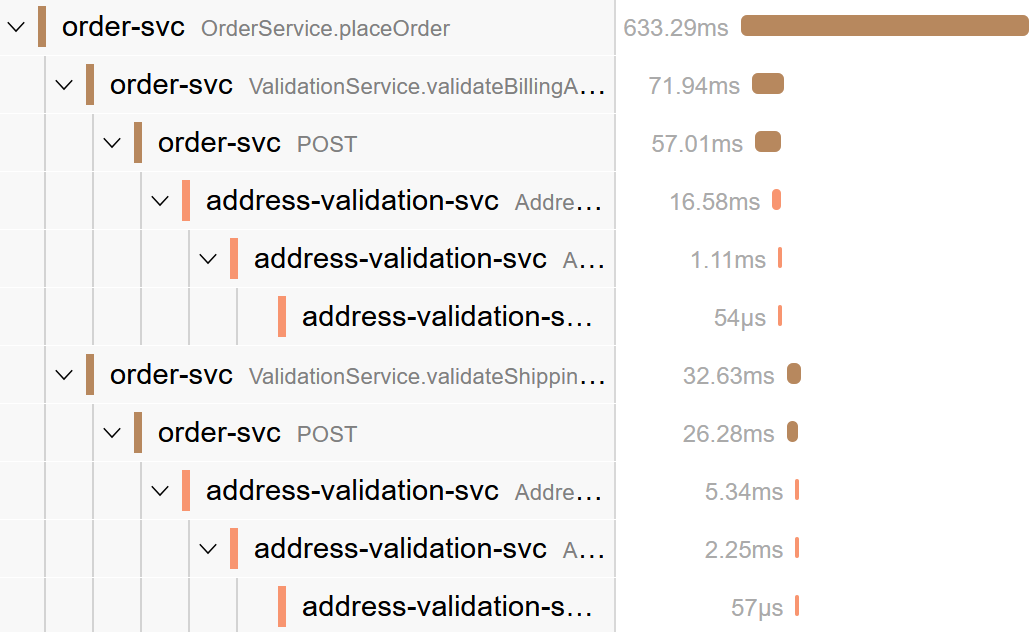
\includegraphics[width=\linewidth]{img/04_erstellung-poc/implementierung_jaeger-trace-example.png}
\caption{Ausschnitt des Traces zu \autoref{lst:implementierung-traced-example}}
\label{fig:implementierung_jaeger-trace-example}
\end{wrapfigure}

In Jaeger erzeugt der o. g. Quellcode die in \autoref{fig:implementierung_jaeger-trace-example} zu sehenden Spans. Bei diesem Ausschnitt ist erkennbar, dass der Dienst \enquote{Bestellungen} für eine ursprüngliche Anfrage zwei Anfragen an den Dienst \enquote{Adressvalidierung} sendet, jeweils für die Rechnungs- und Lieferadresse. Neben den Traces werden keine weiteren Daten von Backend-Komponenten erhoben, da das Hauptaugenmerk der Arbeit auf dem Frontend liegt.

\subsection{Frontend}

\subsubsection{Datenweiterleitung im \enquote{Backend4Frontend}}



Da Logs, Metriken und Fehler mit Splunk gesammelt werden, aber Splunk keine direkt aus dem Browser ansprechbare Schnittstelle bietet, müssen diese über einen Dienst an Splunk weitergeleitet werden (vgl. \autoref{subsec:splunk}). Neben diesen Daten sind zudem Traces auf dem Frontend an Jaeger zu berichten, dies ist aber erneut nicht möglich, da kein browserkompatibler Jaeger-Client identifiziert werden konnte. Eine nähere Betrachtung dessen erfolgt im nächsten Abschnitt.

Da der Dienst \enquote{Backend4Frontend} bereits zum Weiterleiten verwendet wird, wurde dieser erweitert, sodass er Traces, Logs, Metriken sowie Fehler entgegennehmen kann und diese an Jaeger bzw. Splunk sendet. Vor der eigentlichen Weiterleitung werden die Daten mit Kontextinformationen angereichert, wie bspw. der User-IP oder der Browserversion. Die Traces werden dann über eine OpenTelemetry-Anbindung an Jaeger gesendet, die anderen Daten werden an die HEC-Schnittstelle \cite{SplunkHEC} von Splunk übertragen.

\subsubsection{Traces und Metriken}
\label{subsec:traces-und-metriken}

Das Frontend erhebt ebenso wie das Backend Traces, zusätzlich werden aber auch Metriken, Logmeldungen und Fehler erfasst und gemeldet. Traces und Metriken werden auf Basis von OpenTelemetry-JavaScript-Komponenten \cite{OpenTelemetryJS} erhoben. Diese Komponenten werden in einem eigenen Angular-Modul (siehe \autoref{lst:app-observability}) initialisiert und der Anwendung über \enquote{providers} zur Verfügung gestellt. Hierbei wird der SPA ein \texttt{Tracer} bereitgestellt, mit dem Spans aufgezeichnet werden können, ein \texttt{Meter}, welcher es erlaubt Metriken zu erstellen, und eine \texttt{requestCounter}-Metrik, welches die Aufzeichnung der Aufrufanzahl schnittstellenübergreifend erlaubt.

\lstinputlisting[
  language = JavaScript,
     style = ES6,
basicstyle = {\footnotesize\fontfamily{pcr}\selectfont},
   caption = Quellcode des Moduls \enquote{app-observability.module.ts},
captionpos = b,
     label = lst:app-observability
]{content/04_erstellung-poc/implementierung-code/app-observability.module.ts}

Im folgenden \autoref{lst:shopping-cart-datasource} ist die Benutzung des zur Verfügung gestellten \texttt{Tracers} zu sehen, hierbei wird ein Span erstellt und bei Schnittstellenaufrufen an die jeweiligen Services übergeben. Wie der Span weiterverwendet wird, ist im nächsten Absatz beschrieben.

\lstinputlisting[
  language = JavaScript,
     style = ES6,
basicstyle = {\footnotesize\fontfamily{pcr}\selectfont},
   caption = Datenquelle zum Abrufen und Zusammenführen der Artikeldaten,
captionpos = b,
     label = lst:shopping-cart-datasource
]{content/04_erstellung-poc/implementierung-code/tracing_shopping-cart-datasource.ts}

Beispielhaft im Dienst zum Abrufen der Übersetzungsdaten (vgl. \autoref{lst:localization.service}) wird der übergebene Span als Elternspan benutzt. Bei dem eigentlichen HTTP-Aufruf wird zudem ein HTTP-Header \texttt{uber-trace-id} angereichert, den der dort laufende Jaeger-Client interpretiert \cite{JaegerClient} und daraus die Beziehung zu den Frontend-Spans herstellt. Zusätzlich zum Tracing wird hierbei auch die Metrik \texttt{requestCounter} inkrementiert.

\lstinputlisting[
  language = JavaScript,
     style = ES6,
basicstyle = {\footnotesize\fontfamily{pcr}\selectfont},
   caption = Service zum Abrufen der Übersetzungsdaten,
captionpos = b,
     label = lst:localization.service
]{content/04_erstellung-poc/implementierung-code/tracing_localization.service.ts}

Um das Erheben von Traces und Metriken im Frontend zu realisieren, wurden OpenTelemetry-Komponenten herangezogen, da wie in \autoref{subsec:opentelemetry} beschrieben, OpenTelemetry einen vielversprechenden Standard darstellt. Weiterhin konnte keine Bibliothek identifiziert werden, die die Traces erhebt und direkt an Jaeger sendet. Es gibt zwar einen Jaeger-Client für Node.js\footnote{Jaeger-Client für Node.js: \url{https://github.com/jaegertracing/jaeger-client-node}}, jedoch befindet sich das browserkompatible Pendant\footnote{Jaeger-Client für Browser: \url{https://github.com/jaegertracing/jaeger-client-javascript/}} seit 2017 in den Startlöchern \cite{JaegerJSClientUsageInABrowser}. Zudem existiert ein OTel-Exporter für Jaeger\footnote{OTel Jaeger Exporter: \url{https://github.com/open-telemetry/opentelemetry-js/tree/main/packages/opentelemetry-exporter-jaeger}}, welcher jedoch auch nur mit Node.js funktioniert. Grund hierfür ist, dass das zugrundeliegende Protokoll gRPC \cite{grpc} nicht komplett aus einer Browserumgebung aus unterstützt wird \cite{grpcWebLimitations}.

\nomenclature[Fachbegriff]{gRPC}{gRPC Remote-Procedure-Call}

Die gesammelten OTel-Tracingdaten werden über einen Standard-Exporter an das \enquote{Backend4Frontend} gesendet, welcher diese dann in ein Jaeger-konformes Format umwandelt und sie dann subsequent an Jaeger übertragt. Die Metrikdaten werden bereits im Frontend in ein Splunk-kompatibles Logformat konvertiert. Nach der Konvertierung werden die Daten an den \texttt{SplunkForwardingService} übergeben, welcher in \autoref{subsec:weiterleitung-an-splunk} näher beschrieben wird.

\subsubsection{Logging}

Das Logging im Frontend wurde über das npm \cite{NPM} Paket \texttt{ngx-logger}\footnote{ngx-logger auf GitHub: \url{https://github.com/dbfannin/ngx-logger}} realisiert, welches eine speziell an Angular angepasste Logging-Lösung darstellt. Da dieses Paket extra an Angular angepasst ist, lässt es sich ohne großen Aufwand als Modul einbinden und einsetzen (vgl. \autoref{lst:logging_app.module}).

\lstinputlisting[
  language = JavaScript,
     style = ES6,
basicstyle = {\footnotesize\fontfamily{pcr}\selectfont},
   caption = Ausschnitt des Hauptmoduls \texttt{app.module.ts},
captionpos = b,
     label = lst:logging_app.module
]{content/04_erstellung-poc/implementierung-code/logging_app.module.ts}

Wie in den vorherigen Codebeispielen zum Tracing zu sehen war, kann ein \texttt{NGXLogger} im Konstruktor von Komponenten und Diensten injected werden. Logmeldungen, die hiermit erfasst werden, werden je nach Konfiguration und Loglevel der jeweiligen Meldung in die Browserkonsole geschrieben. Über einen \texttt{NGXLoggerMonitor} lassen sich die Logmeldungen anzapfen, wie in \autoref{lst:splunk-logging-monitor} zu sehen ist. Hierbei werden die Logmeldungen in ein Splunkformat übertragen und dann über den \texttt{SplunkForwardingService} an das \enquote{Backend4Frontend} übertragen. Die Funktionsweise der Weiterleitung wird an späterer Stelle genauer beschrieben.

\lstinputlisting[
  language = JavaScript,
     style = ES6,
basicstyle = {\footnotesize\fontfamily{pcr}\selectfont},
   caption = Implementierung des \texttt{NGXLoggerMonitor}-Interfaces,
captionpos = b,
     label = lst:splunk-logging-monitor
]{content/04_erstellung-poc/implementierung-code/splunk-logging-monitor.ts}

\subsubsection{Fehler}

Die ErrorHandler-Hook von Angular übermittelt aufgetretene und unbehandelte Fehler an den \texttt{SplunkForwardingErrorHandler}. Weiterhin ist der ErrorHandler ein \texttt{Injectable}, wodurch er in andere Angular-Klassen \enquote{injected} werden kann. Der ErrorHandler wird bspw. bei den Schnittstellen dazu verwendet, um dort bereits behandelte Fehler auch an Splunk zu übermitteln.

Wird ein Fehler gemeldet, werden zunächst die Fehlerinformationen in einen Splunk\-da\-ten\-satz konvertiert und dann über den \texttt{SplunkForwardingService} weitergeleitet. Neben diesem Verhalten wird zusätzlich auch der Fehler an LogRocket übermittelt, damit dieser im Video des Session-Replays gesondert angezeigt wird.

\lstinputlisting[
  language = JavaScript,
     style = ES6,
basicstyle = {\footnotesize\fontfamily{pcr}\selectfont},
   caption = ErrorHandler zum Abfangen und Weiterleiten von aufgetretenen Fehlern,
captionpos = b,
     label = lst:splunk-forwarding-error-handler
]{content/04_erstellung-poc/implementierung-code/splunk-forwarding-error-handler.ts}

\subsubsection{Weiterleitung an Splunk}
\label{subsec:weiterleitung-an-splunk}

Logs, Metriken und Fehler über den  \texttt{SplunkForwardingService} an das \enquote{Backend\-4\-Frontend} gesendet und letztendlich an Splunk übermittelt. Damit nicht jedes Datenobjekt einen Aufruf auslöst, gruppiert dieser \texttt{Service} die eintreffenden Daten.

Im \autoref{lst:splunk-forwarding.service} ist erkennbar, dass alle 5s geprüft wird, ob Daten zur Weiterleitung zur Verfügung stehen. Ebenso ist zu sehen, dass beim Fehlschlag des Sendens eines Batches, fünf Wiederholversuche gestartet werden, mit einer Wartezeit von 15s. Die grundlegende Funktionalität dessen wurde mit RxJS \cite{RxJS} umgesetzt, einer Kernbibliothek von Angular, die Reactive Programming \cite{ReactiveProgramming} in JavaScript erlaubt. Weiterhin werden die Daten an Splunk nicht im Textformat übertragen, sondern direkt in JSON. Die JSON-Objekte werden automatisch von Splunk interpretiert und die enthaltenen Felder zugreifbar gemacht. Durch das gewählte Format \cite{StructuredAndInteroperableLogging} ist auch die \autoref{anf:3200} zum Structured-Loggings erfüllt. Ausgesuchte Logmeldungen und Fehler sind in \autoref{lst:log-batch_example} zu betrachten.

\lstinputlisting[
  language = JavaScript,
     style = ES6,
basicstyle = {\footnotesize\fontfamily{pcr}\selectfont},
   caption = Implementierung des \texttt{SplunkForwardingService},
captionpos = b,
     label = lst:splunk-forwarding.service
]{content/04_erstellung-poc/implementierung-code/splunk-forwarding.service.ts}

\pagebreak

\lstinputlisting[
  language = JSON,
basicstyle = {\footnotesize\fontfamily{pcr}\selectfont},
   caption = Beispiel eines Batches,
captionpos = b,
     label = lst:log-batch_example
]{content/04_erstellung-poc/implementierung-data/log-batch_example.json}

\subsubsection{Session-Replay}

\begin{wrapfigure}[9]{r}{0.35\textwidth}
\centering
\vspace{-0.5\baselineskip}
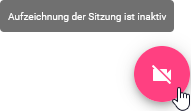
\includegraphics[width=\linewidth]{img/04_erstellung-poc/implementierung_frontend_recording-consent_button-inactive.png}
\caption{Button zum Öffnen des Dialogs}
\label{fig:recording-consent_button-inactive}
\end{wrapfigure}

Die Übermittlung der Daten an LogRocket wird erst aktiviert, wenn der Nutzer explizit der Aufzeichnung zustimmt. Dies bedeutet jedoch auch, dass bis zur Zustimmung keine Sitzungsdaten aufgenommen wurden. Klickt der Nutzer jedoch auf den, unten rechts in der Anwendung schwebenden, Button (vgl. \autoref{fig:recording-consent_button-inactive}), wird ein Einverständnis-Dialog geöffnet. Hierbei (vgl. \autoref{fig:recording-consent_dialog-inactive}) erhält der Nutzer eine Übersicht welche Daten aufgenommen werden und an wen diese dann weitergesendet werden. Stimmt der Nutzer zu, wird LogRocket initialisiert, wie im \autoref{lst:record-consent-dialog.component.html} sowie \autoref{lst:record-consent-dialog.component.ts} zu sehen ist. Nach dem Warenkorbdialog und nach der Eingabe der Rechnungsadresse werden zudem weitere identifizierende Daten an LogRocket übermittelt. Die Aufnahme der Sitzung läuft größtenteils autonom, lediglich behandelte Fehler müssen LogRocket manuell übermittelt werden.
	
\begin{figure}[H]
	\centering
	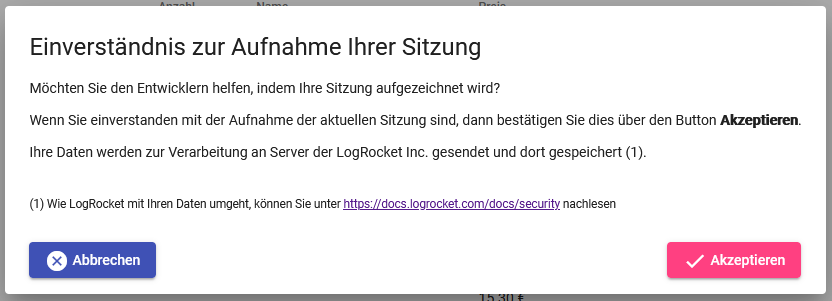
\includegraphics[width=1.00\linewidth]{img/04_erstellung-poc/implementierung_frontend_recording-consent_dialog-inactive.png}
	\caption{Einverständnis-Dialog}
	\label{fig:recording-consent_dialog-inactive}
\end{figure}

\vspace{-0.5\baselineskip}

\lstinputlisting[
  language = AngularTemplateHTML,
basicstyle = {\footnotesize\fontfamily{pcr}\selectfont},
   caption = Angular HTML-Template der Einverständnis-Komponente,
captionpos = b,
     label = lst:record-consent-dialog.component.html
]{content/04_erstellung-poc/implementierung-code/record-consent-dialog.component.html}

\lstinputlisting[
  language = JavaScript,
     style = ES6,
basicstyle = {\footnotesize\fontfamily{pcr}\selectfont},
   caption = Initialisierung von LogRocket in der Einverständnis-Komponente,
captionpos = b,
     label = lst:record-consent-dialog.component.ts
]{content/04_erstellung-poc/implementierung-code/record-consent-dialog.component.ts}

\subsection{Architektur}

Abschließend lässt sich somit folgende, in \autoref{fig:implementierung_architektur} zu betrachtende, Architektur visualisieren. Bei \circled{1} lässt sich die Übertragung von Spans an Jaeger betrachten, bei dem die Backend-Dienste aufgrund der verwendeten Java-Anbindung (\texttt{io\allowbreak{}.\allowbreak{}jaegertracing\allowbreak{}:\allowbreak{}jaeger-client}) die Spans über das Protokoll \enquote{Apache Thrift} \cite{Thrift} berichten und das \enquote{Backend4Frontend} verwendet zur Weiterleitung eine OTel-Anbindung an Jaeger, die wiederum gRPC verwendet. Die Übertragung von Log-, Metrik sowie Fehlerdaten lässt sich bei \circled{2} betrachten. Dabei handelt es sich um Daten, die zuvor vom Frontend gesendet wurden (vgl. \circled{3}). Die Kommunikation mit LogRocket (vgl. \circled{4}) verläuft ohne Weiterleitung und mit einem proprietärer Protokoll auf Basis von gRPC \cite{LogRocketPerformance}.

\pagebreak

\begin{figure}[H]
	\begin{adjustbox}{addcode={
		\begin{minipage}{\width}}{
			\caption{Architektur des Proof-of-Concepts. Eigene Darstellung}
			\label{fig:implementierung_architektur}
		\end{minipage}},rotate=90,center}
		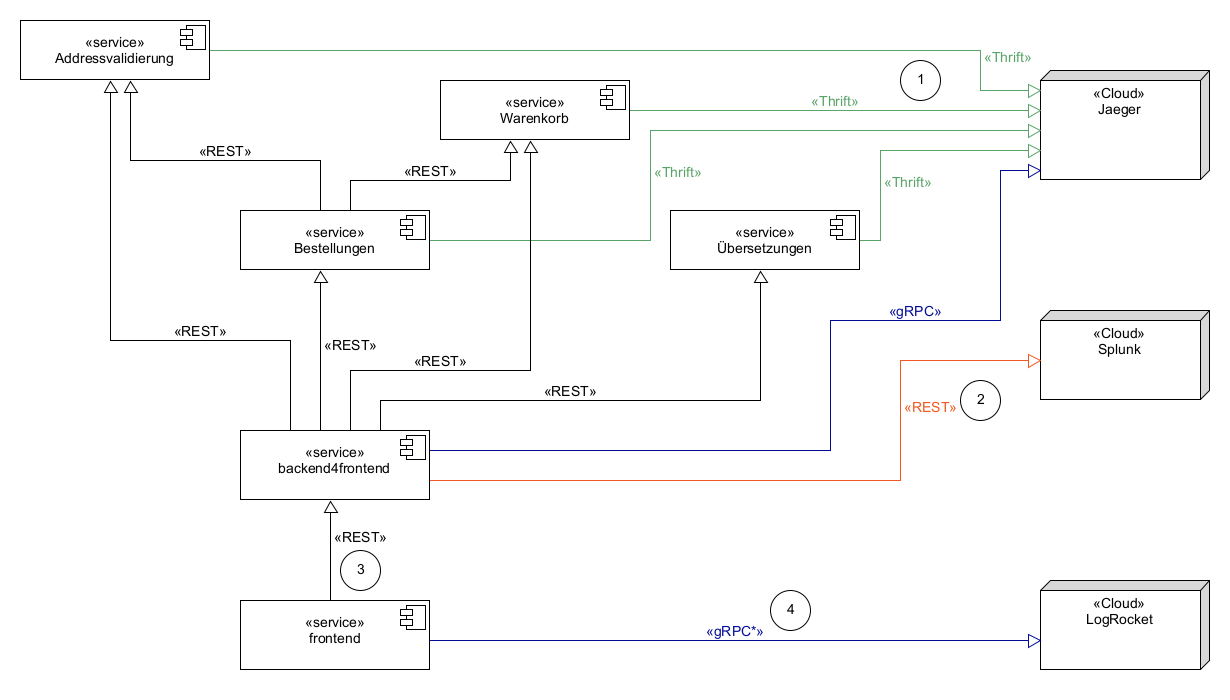
\includegraphics[height=0.80\textwidth]{img/04_erstellung-poc/implementierung.png}
	\end{adjustbox}
\end{figure}

\pagebreak